\chapter{映像伝送システム}
\label{chap:video-transmission}

\section{ビデオカメラ}
\label{sec:camera}


\section{ディスプレイ}
\label{sec:display}


\section{インターレース}
\label{sec:interlace}


\section{色空間}
\label{sec:colorspace}

一般的に液晶ディスプレイでは、1ピクセルを赤、緑、青、すなわちRGBの3つの色信号で表現する。多くのPCやゲーム機の出力では、RGBの色空間が使われる。
% 多くのPCやゲーム機の出力では、RGBそれぞれに8bitで表現するため、1ピクセルあたり24bitとなり、16,777,216色を表現することができる。

一方、ビデオカメラでは、輝度信号Yと、2つの色差信号を使って表現される色空間であるYUVが使われるが多い。[要出典]
この方式の特徴は、「人間の目は明るさの変化には敏感だが、色の変化には鈍感である」という性質に基づいて、色度信号の情報量を減らすことができるという点にある。

\begin{figure}[htbp]
    \begin{center}
        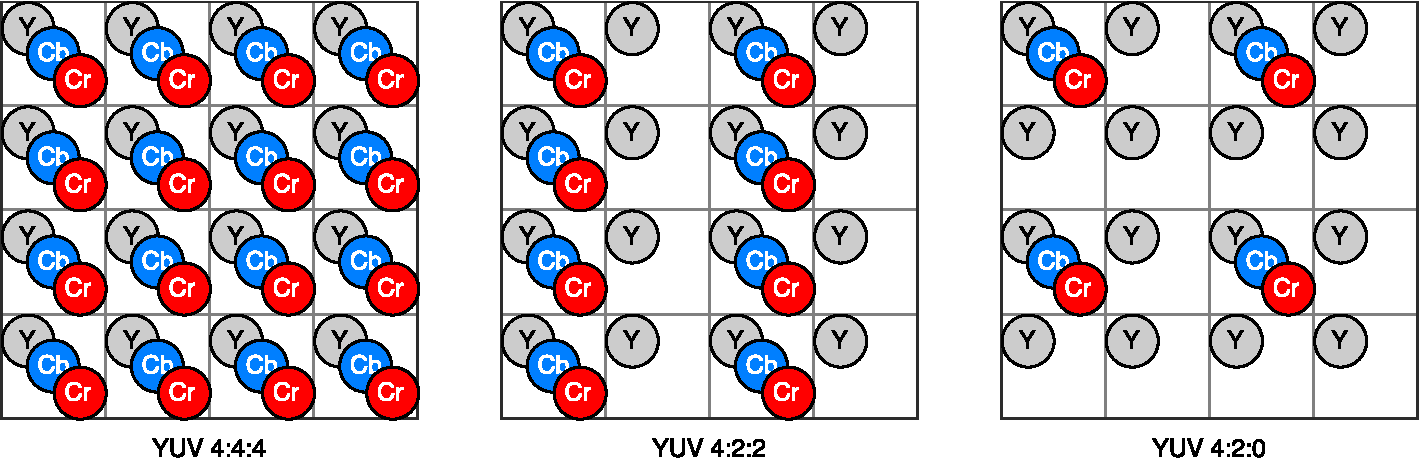
\includegraphics[bb=0 0 681 222,width=14cm]{img/yuv-pixel-structure.pdf}
    \end{center}
    \caption{YUVのピクセルあたりの色情報の構造}
    \label{fig:yuv-pixel-structure}
\end{figure}

% YUVのピクセルあたりの色情報の構造を、図\ref{fig:yuv-pixel-structure}に示す。

YUV 4:4:4では、輝度信号、色差信号共に1ピクセル毎である。
YUV 4:2:2では、輝度信号は1ピクセル毎、色差信号は2ピクセル毎であり、YUV 4:4:4と比べ、帯域はおよそ2/3となる。
YUV 4:2:0では、輝度信号は1ピクセル毎、色差信号は4ピクセル毎であり、YUV 4:2:2と比べ、帯域はおよそ3/4となり、YUV 4:4:4と比べ、帯域はおよそ1/2となる。

\section{帯域}
\label{sec:bandwidth}

帯域は次のようになる。

帯域は解像度の他にも、インターレース、色空間、色深度により変化する。

表は次のように出力される。(表\ref{tb:video-bandwidth})

\begin{table}[htbp]
  \caption{解像度、フレームレート、色空間による帯域の変化}
  \label{tb:video-bandwidth}
  \begin{center}
  \begin{tabular}{c|c|c|c|c}
    \hline
    解像度     & フレームレート & 色空間 & ピクセルあたりのビット数 & 帯域\\\hline\hline
    3840x2160 & 60p          & RGB    & X bit               & XX Gbps\\\hline
    3840x2160 & 30p          & RGB    & X bit               & XX Gbps\\\hline
    3840x2160 & 30p          & RGB    & X bit               & XX Gbps\\\hline
    3840x2160 & 30p          & YUV444 & X bit               & XX Gbps\\\hline
    3840x2160 & 30p          & YUV422 & X bit               & XX Gbps\\\hline
    3840x2160 & 30p          & YUV420 & X bit               & XX Gbps\\\hline
    1920x1080 & 60p          & RGB    & X bit               & XX Gbps\\\hline
    1920x1080 & 60i          & YUV    & X bit               & XX Gbps\\\hline
    1920x1080 & 60i          & YUV    & X bit               & XX Gbps\\\hline
  \end{tabular}\end{center}
\end{table}

\section{インターフェース}
\label{sec:interface}

\subsection{VGA}

\subsection{DVI}

\subsection{HDMI}
1.4 / 2.0

\subsection{SDI}


% \begin{table}[htbp]
%   \caption{解像度、フレームレート、色空間による帯域の変化}
%   \label{tb:hdmi-feature}
%   \begin{center}
%   \begin{tabular}{c|c|c|c|c}
%     \hline
%               & HDMI 1.4 & HDMI 2.0 \\\hline\hline
%     3840x2160 & 60P          & RGB    & X bit               & XX Gbps\\\hline
%     3840x2160 & 30P          & RGB    & X bit               & XX Gbps\\\hline
%     3840x2160 & 30P          & RGB    & X bit               & XX Gbps\\\hline
%     3840x2160 & 30P          & YUV444 & X bit               & XX Gbps\\\hline
%     3840x2160 & 30P          & YUV422 & X bit               & XX Gbps\\\hline
%     3840x2160 & 30P          & YUV420 & X bit               & XX Gbps\\\hline
%     1920x1080 & 60P          & RGB    & X bit               & XX Gbps\\\hline
%     1920x1080 & 60P          & YUV    & X bit               & XX Gbps\\\hline
%     1920x1080 & 30P          & RGB    & X bit               & XX Gbps\\\hline
%   \end{tabular}\end{center}
% \end{table}

\section{伝送手法}

\section{まとめ}
